\documentclass[tikz,border=4pt]{standalone}
\usepackage{tikz}
\begin{document}
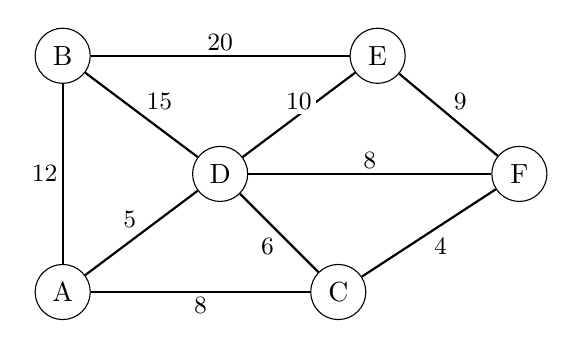
\begin{tikzpicture}[
  vertex/.style={circle,draw,minimum size=7mm,inner sep=0pt},
  edge/.style={line width=0.8pt},
  weight/.style={fill=white,inner sep=1.5pt,font=\small}
]
\node[vertex] (A) at (0,0) {A};
\node[vertex] (B) at (0,3) {B};
\node[vertex] (D) at (2,1.5) {D};
\node[vertex] (C) at (3.5,0) {C};
\node[vertex] (E) at (4,3) {E};
\node[vertex] (F) at (5.8,1.5) {F};

\draw[edge] (A)--node[weight,left]{12}(B);
\draw[edge] (A)--node[weight,above left]{5}(D);
\draw[edge] (A)--node[weight,below]{8}(C);
\draw[edge] (B)--node[weight,above right]{15}(D);
\draw[edge] (B)--node[weight,above]{20}(E);
\draw[edge] (D)--node[weight,above]{10}(E);
\draw[edge] (D)--node[weight,above]{8}(F);
\draw[edge] (D)--node[weight,below left]{6}(C);
\draw[edge] (E)--node[weight,above right]{9}(F);
\draw[edge] (C)--node[weight,below right]{4}(F);
\end{tikzpicture}
\end{document}
